\subsection{研究意义}

云南省与缅甸、老挝、越南三国接壤,边境线长达4060公里,边境地区山川秀丽,被誉为“植物王国”和“世界花园”。
然而,边境地区地形复杂多变,山地、高原、河谷等地貌交错分布且缺乏天然屏障,使得边境地区长期以来存在严重的非法越境隐患。
非法越境问题主要表现为人口非法流动、毒品走私、货物走私以及跨境犯罪等多种形式,该问题不仅直接影响边境地区的安全与稳定,还可能引发跨境犯罪、社会矛盾和民族问题,进而威胁国家整体安全和社会秩序。
近年来,云南边境地区非法越境问题愈发突出,给边境地区的社会稳定和国家的长治久安带来了巨大压力,见图。
2020年至2021年期间,张某、匡某等11人不顾疫情防控政策,为获取高额报酬,违反出入国(边)境管理法规,采取带路爬山、以摩托和轿车交互运输、用货物遮挡、绕道小路等方式逃避检查,组织、运送大批人员非法出、入境,更有涉案人员趁机实施运输毒品犯罪,严重破坏国(边)境管理和疫情防控工作\footnote{信息来源:云南长安网(\url{https://www.yncaw.gov.cn/html/2022/ftnw_0226/87066.html})}。
2022年,云南警方破获了一起特大组织、运送他人偷越国(边)境案件,摧毁了一个涉及12个省市的犯罪网络,累计抓获485名涉案人员。该犯罪团伙通过发布虚假的高薪务工信息,诱骗境内人员前往云南边境,再通过分段运输的方式将其非法运送出境\footnote{信息来源:云南网(\url{https://m.thepaper.cn/baijiahao_17977737})}。
2023年8月15日,一名22岁云南女大学生李某被传疑似被拐卖至缅北。相关消息在社交平台上引发关注,但经警方调查,李某最终被找到\footnote{信息来源:澎湃新闻(\url{https://mp.weixin.qq.com/s/rDFU-b5pEK7kuw1zO5EQxA})}。
上述案件类型反映出云南边境地区在打击非法越境问题方面仍面临挑战,但同时也显示了执法部门在追捕犯罪嫌疑人和保护受害者方面的积极努力。

\begin{figure}[h!]
\centering %图片居中
\subfloat[``1·24"非法越境案件]{
	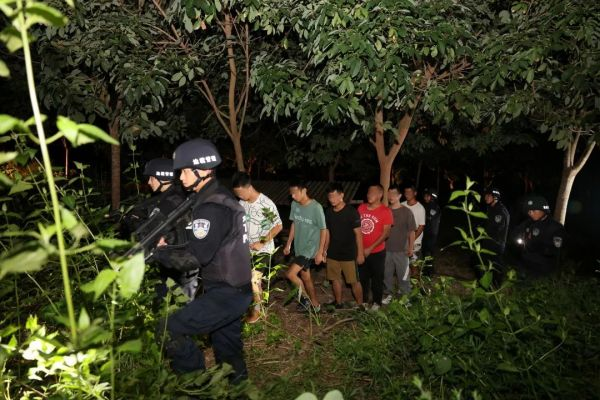
\includegraphics[width=0.35\textwidth]{1}
}
\subfloat[2022特大非法越境案件]{
	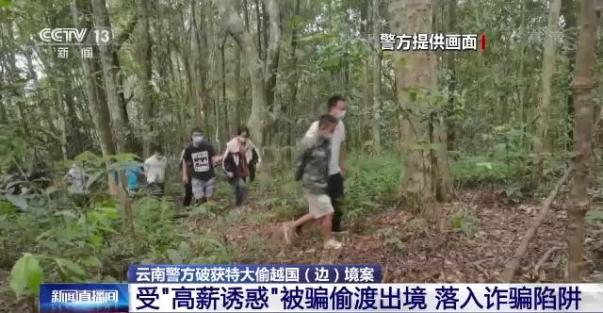
\includegraphics[width=0.45\textwidth]{2}
}\\
% \subfloat[演员王星被拐前形象]{
% 	
\includegraphics[width=0.3\textwidth]{1-1}
% }
% \subfloat[演员王星被拐后照片]{
% 	
\includegraphics[width=0.3\textwidth]{1-2}
% }
\captionsetup{justification=centering} %图题居中
\caption{近年云南非法越境案件}
\label{fig:case-}
\end{figure}

打击非法越境是一个大场景下全天候的目标监控任务,监控系统需要在较大地理空间范围上对目标进行监控,还需要实现7x24小时风全气候条件下的监控覆盖。边境公安针对该问题正积极探索并应用前沿监控技术,以替代传统的警员巡逻模式,旨在克服传统手段中巡逻覆盖范围有限、反应速度滞后以及难以实现全天候、全方位监控等固有缺陷,同时有效应对日益隐蔽化和智能化的非法过境手段。然而,现有监控设备在技术层面仍存在显著不足,特别是缺乏高科技手段(如智能识别系统、多光谱成像、无人机协同巡查等)的深度集成,导致对非法过境行为的精准识别与打击能力未能达到预期效果。例如:
\begin{itemize}[left=15pt,label={\textasteriskcentered}]
\item 现有监控设备在多样化地形环境中的适应性存在不足。边境地区地形复杂多样,涵盖高山、丛林、河流等多种地貌,且环境动态变化频繁,这使得现有设备对环境的感知能力受限,难以同时适应不同的地形地貌,并难以有效处理环境内物体随天气、时间变化导致的光线、能见度,以及物体形态等方面的变化;
\item 现有监控设备对大场景内的潜在目标主动预测与定位能力表现不足。具体而言,现有系统主要依赖被动式监控,缺乏基于数据分析的主动预测机制,无法对非法越境目标的出现位置、行为轨迹及潜在风险进行实时预测与精准预判。这一技术短板导致边境安防工作处于被动监控模式,难以在非法活动发生前采取有效干预措施,从而降低了整体防控效能;
\item 现有监控设备处在小范围监控模式下,大场景下的监控部署与运维成本居高不下。由于现有监控设备主要依赖于被动式监控模式,单一摄像头监控范围严重受限,对云南省4060公里长的边境地区无缝铺设监控设备将带来巨大的前期投入和后期运维成本。另外,现有监控设备缺乏基于人工智能算法和多源数据融合的主动搜索机制,无法通过调整摄像头俯仰角、转动角及焦距主动发现边境大场景下的目标,摄像头往往处于固定的监控区域或通过人力进行调整,这种监控范围上的限制进一步制约了整体防控效能的提升。
\end{itemize}
这些技术瓶颈不仅制约了边境管理效能的提升,也为非法越境活动提供了可乘之机,亟需通过技术创新与系统优化加以突破。


本项目旨在通过运用大数据分析与机器学习技术,将人工干预的被动监控模式转变为算法实时控制的主动预测与搜索模式,提升监控设备在大场景下的自主监控能力,从而有效治理非法越境问题,保障国家主权安全,推动边疆地区经济社会发展,为国家的稳定和发展创造良好环境。


\subsection{国内外研究现状及发展动态分析}




不足:
1. 监控设备无法有效应对超大场景中物体形态、位置和光照等因素的变化,即使较为微小的变化也可能导致监控无法正确提取场景特征
2. 在边境线形成的超大场景中,监控设备的选址往往较为固定,不能动态的调整和监控目标出现概率大的区域
3. 无法主动在大场景下通过调整摄像设备的转角、俯仰、和焦距以自动搜索目标,非常依赖大量警力定时定点巡逻,午夜往往会形成监控盲区和漏洞

挑战:
1. 大场景下现有模型训练与迁移成本与场景数量成比例增加
2. 
3. 覆盖大场景搭建与运维成本太过巨大

内容:
1. 图片特征泛化
2. 动态图预测
3. 大场景主动搜索

科学问题:
1. 大场景图像到图的转化及其表示学习,使得模型摆脱对图像局部数据的单一依赖
2. 
3.

首先,云南边境地区地形复杂,涵盖高山、丛林、河流等多种地貌,不同的景观设的自动化监控设备不能有效获取

许多区域人迹罕至,难以实现全面覆盖的监控网络,这为非法越境活动提供了天然的隐蔽条件。

其次,边境线长达4060公里,现有的监控设施和技术手段难以满足全天候、全方位的监控需求,尤其是在偏远地区,监控盲区较多,导致非法越境活动有机可乘。

最后,边境安防资源的分配不均衡,边防力量、资金和设备的投入有限,难以应对日益复杂和隐蔽的非法越境手段。例如,部分边境区域缺乏先进的监控设备(如红外探测、无人机巡逻等),导致对非法越境活动的实时监测和快速响应能力不足。这些安防监控的不足不仅加剧了非法越境问题的复杂性,也对边境地区的安全治理提出了更高的要求。因此,加强边境安防监控技术的研发与应用,优化资源配置,构建智能化、立体化的监控体系,是解决非法越境问题的关键路径之一。
















导致云南边境非法越境问题的原因是多方面的,涉及地理、经济、社会、政治等多个维度。首先,地理因素是非法越境问题的重要诱因。云南边境地形复杂,许多区域人迹罕至,难以实施全面监控,加之边境线漫长,有限的边防力量难以覆盖所有区域,这为非法越境活动提供了可乘之机。其次,经济发展不平衡是非法越境问题的重要驱动因素。云南边境地区与邻国如缅甸、老挝的经济发展水平存在较大差距,部分邻国居民为改善生活条件,选择非法进入中国。同时,边境地区部分居民生活贫困,容易受到非法活动的诱惑,参与走私、偷渡等行为。社会与文化因素也在其中扮演了重要角色。云南边境地区居住着多个跨境民族,如傣族、景颇族等,他们与邻国居民在语言、文化、血缘上有着密切联系,这种跨境联系为非法越境提供了便利。此外,部分边境地区社会治理能力薄弱,基层管理存在漏洞,难以有效遏制非法活动。

政治与法律因素同样不可忽视。邻国如缅甸长期存在政治动荡和武装冲突,导致大量难民和非法移民涌入云南边境,进一步加剧了非法越境问题的复杂性。跨境犯罪活动往往涉及多国,法律管辖和执法合作存在困难,难以形成有效的打击合力。技术与资源的限制也是边境管理面临的重要挑战。边境地区监控设施和技术手段相对落后,难以实现全天候、全方位的监控,而边防力量、资金和设备的分配也难以满足实际需求,导致部分边境区域管理薄弱。

云南边境非法越境问题不仅是一个区域性问题,更是涉及国家安全、社会稳定、经济发展和生态保护的综合性挑战。深入研究这一问题具有重要的理论和现实意义。从理论角度来看,通过多学科交叉研究,可以构建边境非法越境问题的理论框架,丰富边境治理和跨境管理的理论研究。从现实角度来看,研究成果可为政府制定边境管理政策、优化资源配置、提升治理能力提供科学依据,有助于维护边境安全、促进区域经济发展和社会稳定。因此,针对云南边境非法越境问题的研究具有重要的科学价值和社会意义。













免责声明:敬请大家仔细对比本模版与官方word转pdf后的差别,自行确定是否采用。
取消正文tex这一行注释即可对比:\verb|%\renewcommand{\input}[1]|\\
\verb|{\vspace{\baselineskip}}|。
个人认为,2025年系统仍然上传PDF,只要人眼无法分辨与官方区别,就可以。

\subsection{编译方法}
\begin{enumerate}
	\item 编译:XeLaTex->bibtex->XeLaTeX->XeLaTeX
	\item 排错:多看编译错误,多查询错误解决方法;编译警告,只要不影响PDF,就不用管。本模版多人使用,可以认为不存在编译错误。
	\item 自定义格式:多阅读一下nsfc.sty,可以解决你绝大部分问题。超过nsfc.sty范围的,建议不要想办法定制,事倍功半。
\end{enumerate}


\subsection{编辑方法}
%%%%%%%%
%\newpage
\vspace{-5pt}

\begin{figure}[h!]
	\centering %图片居中
	\includegraphics[width=6cm]{figures/xiugai.png}
	\captionsetup{justification=centering} %图题居中
	\caption{项目文件夹结构}
\end{figure}
只需要修改上图中蓝色选中区域文件即可。其他剩余文件,可以直接采用模版替换,编译就是最新版。

\subsubsection{章节}\label{subsubsec:t}
\verb|\label{subsubsect:t}|
引用章节\verb|\ref{subsubsec:t}|,生成为:\ref{subsubsec:t}。这个样式可能不是你想要的,那种情况下,就手敲吧!申请书不像论文,这种情况应该没几个。

\subsubsection{字体}
中文\textbf{粗体};\textbf{bold} font;
中文\textit{斜体};\textit{italic} font;

克制使用以下标注(不用更好),防止专家眼花缭乱。\textul{添加下划线};\textull{添加双下划线};\textuw{添加下弯线};\textud{添加下点线}。

全文改宋体,可以修改nsfc.sty的MS部分字体。

可选的就是\verb|\zhkai,\enkai,\zhsong,\ensong|。

\subsubsection{文献}
普通引用\cite{test};上标引用\citess{test};多篇文章\citess{test,test2,test3}。

有注音的英文:\cite{test}。

参考期刊\cite{test};
参考图书\cite{test2};
参考会议\cite{test5};
参考链接\cite{test4};
参考文件\cite{test6}。

对于中文参考文献,bib条目中需要有language = {zh},参见\cite{test2}。
\subsubsection{列表}
无序列表\footnote{值得注意的是,不需要一定要用列表环境,用加粗、换行、缩进同样能达到效果。
	因为咱们的初衷,还是LaTeX在排版文献和公式上有优势,发挥这一个优势就行了,其他部分不需要强行套用。文本本身还是最重要、需要大家投入精力的部分。}的例子:
\begin{itemize}[left= 50pt]
	\item[-] 第一条,第一条的内容可能很长长长长长长长长长长长长长长长长长长长长;
	\item[-] 第二条。
\end{itemize}

有序列表的例子:
\begin{enumerate}[left= 50pt]
	\item 第一条,第一条的内容可能很长长长长长长长长长长长长长长长长长长长长;
	\item 第二条。
\end{enumerate}

两个带圈文字的实现方法:
\textcircled{\raisebox{-0.8pt}{1}}
\textcircled{\textbf{\small 1}}

注意,由于列表的缩进,不同使用者可能偏向并不一样。本模版用的enumitem包,阅读他的文档进行个性化,其文档在:https://www.ctan.org/pkg/enumitem


\subsubsection{公式}

公式如下:
\begin{equation}
	E=mc^2
\end{equation}
公式的上下间距参见nsfc.sty中公式上下间距部分。

\subsubsection{图}
图片的例子:
\begin{figure}[h!]
\centering %图片居中
\includegraphics[width=2cm]{figures/IMG.JPG}
\captionsetup{justification=centering} %图题居中
\caption{这是图题}
\end{figure}

图题和表头若想取消加粗,去掉nsfc.sty中caption部分的\verb|\bfseries|即可。


\subsubsection{表}
在表格内的第一行设置\verb|\zhkai\ensong\selectfont|,来选择字体。

其中\verb|\zhkai\zhsong\enkai\ensong|可以根据需要选择。
\begin{table}[htbp]
	\zhkai\ensong\selectfont%设置表格字体
	\centering  % 显示位置为中间
	\caption{表格}  % 表格标题
	\label{table1}  % 用于索引表格的标签
	%字母的个数对应列数,|代表分割线
	% l代表左对齐,c代表居中,r代表右对齐
	\begin{tabular}{|c|c|c|c|}  
		\hline  % 表格的横线
		& & & \\[-6pt]  %可以避免文字偏上来调整文字与上边界的距离
		第一列&第二列&第三列&第四列 \\  % 表格中的内容,用&分开,\\表示下一行
		\hline
		& & & \\[-6pt]  %可以避免文字偏上 
		0.1&0.2&0.3&0.4 \\
		\hline
	\end{tabular}
\end{table}

\subsection{某页最后一段行距可能很窄?}
如果没有这个问题,就不用管这个事情。

行间距变化一般是在“多行蓝色模版”部分前后。因为蓝色模版文字在section里写的,latex把蓝色部分当作一个整体,可能硬要挤到这一页,而不是换新一页,导致会挤前一页的行间距,导致前一页行距异常。
针对这种情况,模版已经使用
\begin{lstlisting}[language=tex, basicstyle=\ttfamily\small, keywordstyle=\color{blue}, commentstyle=\color{gray}]
	%自动段落的行间距微调
	\usepackage{setspace}
	\setstretch{1.6} % 22 bp / 14 pt = 1.571
\end{lstlisting}
降低了这种情况发生的可能。
如果还有,就只好添加\verb|\newpage|把它newpage到后一页上,就行了。也可以考虑分段缓解,需要写的时候注意页面的分段和字数。

\begin{REF}
\subsection*{参考文献}
\vspace{-50pt}
\bibliographystyle{template/latex/gbt7714-nsfc}
\bibliography{sections/a6参考文献}%参考文献
\end{REF}

\newpage%自己判断是否需要